% TODO: review/complement the introduction, it is very important for a
% thesis/paper
\chapter{Introduction}\label{chap:introduction}
\section{Background}

The growing demand for energy and the challenges related to climate change
require a transition towards renewable-based generation. Some examples of
environmental requirements are discussed in the Sustainable Development Goals
(SDGs) \cite{sdgs} and the Conference of the Parties (COP) \cite{COP} by the
United Nations. It has been established that global net human-caused emissions
of carbon dioxide ($\text{CO}_2$) need to decrease by approximately 45 percent
from 2010 levels by 2030, reaching net zero around 2050.

As a consequence, the total share of energy generation from renewable sources
has been increasing significantly in recent years. Some studies predict that by
2050, 91\% of electricity generation will come from renewable resources,
primarily solar and wind energy \cite{irena}. These emerging sources come in
various sizes, ranging from residential-scale rooftop systems to utility-scale
power plants, and they are interconnected across the electric grid, linking both
the distribution system and the high-voltage transmission system. Significantly,
for the focus of our study, a considerable number of these new resources connect
to the power system through power electronic inverters\cite{osti}.

Therefore, the transition towards renewable-based generation implies a shift
from large centralized generation units, mainly composed of synchronous
generators (SG), to decentralized/distributed generation units, mainly composed
of inverter-based resources (IBR).

\begin{figure}[h!]
    \centering
    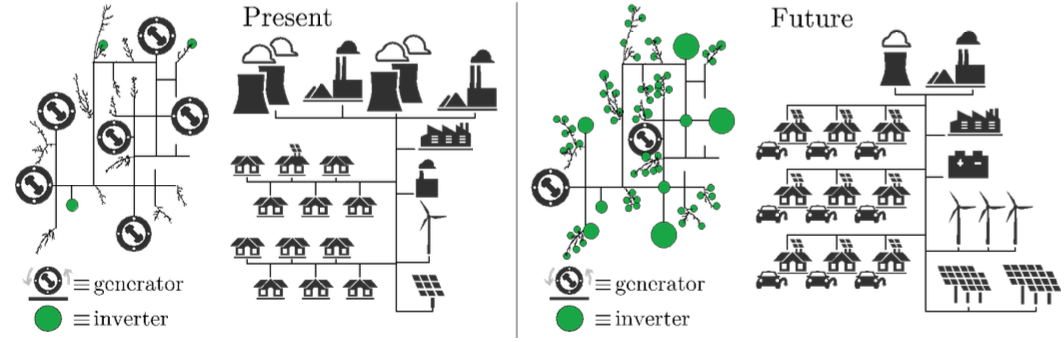
\includegraphics[width=14cm]{images/future_grid.png}
    \caption{Present and future/projected power grids\cite{osti}.}
    \label{fig:future_grid}
\end{figure}

% TODO: include the following sections according to Jia Liu's dissertation.
% \section{Inverter-based resources (IBR)}
% \subsection{Topologies}
% \subsection{Control methods}
% \subsection{Challenges}

However, the replacement of SGs by IBRs has created new challenges for research
related to stability requirements and the reliability and controllability of the
system \cite{alam2020challenges}. Some of the challenges include:

\begin{itemize}
    \item Low inertia and frequency issues
    \item Fault Ride Through (FRT) capability issues
    \item Power quality issues
    \item Uncertainty issues
\end{itemize}

Among the several issues mentioned, the loss of system inertia is the most
detrimental to the power system \cite{alam2020challenges}. System inertia refers
to the kinetic energy of all interconnected SGs of a power
system \cite{denholm2020inertia}. In the case of a sudden increase in load or
loss of generation, the kinetic energy stored in the SGs can bridge the gap
between generation and consumption for a few seconds until a control action
takes corrective measures. Since IBRs rely on electronic devices, they have very
low or no inertia, and substituting SMs with IBRs would lead to a drastic
reduction in the total system inertia.

In addition, today's IBRs generally rely on phase-locked loops (PLLs) to
estimate the voltage angle at the inverter terminals, which is then used to
control the inverter current output using vector control \cite{ndreko2018grid}.
Therefore, these inverters "follow" the grid voltage and frequency, which are
typically generated by SGs, and are called grid-following inverters (GFLI).
Consequently, this control technique only works well in stiff AC grids with low
frequency and voltage deviations.

In summary, the penetration of GFLI-based IBRs in power generation is very
limited, as they have very low inertia and rely on a stiff AC grid. To address
this problem, a new inverter control paradigm called grid-forming control has
been developed. Grid-Forming Inverters (GFMI) act as ideal voltage sources
actively controlling the magnitude of voltage and the frequency at the point of
common coupling (PCC) \cite{pattabiraman2018comparison}.

Consequently, GFMI is expected to facilitate the development of scalable and
decentralized AC power systems, wherein the voltages and frequency are
controlled through the collaborative interactions among the grid-forming units.
The subsequent figure elucidates the primary distinctions between GFMI and GFLI.

\begin{figure}[h!]
    \centering
    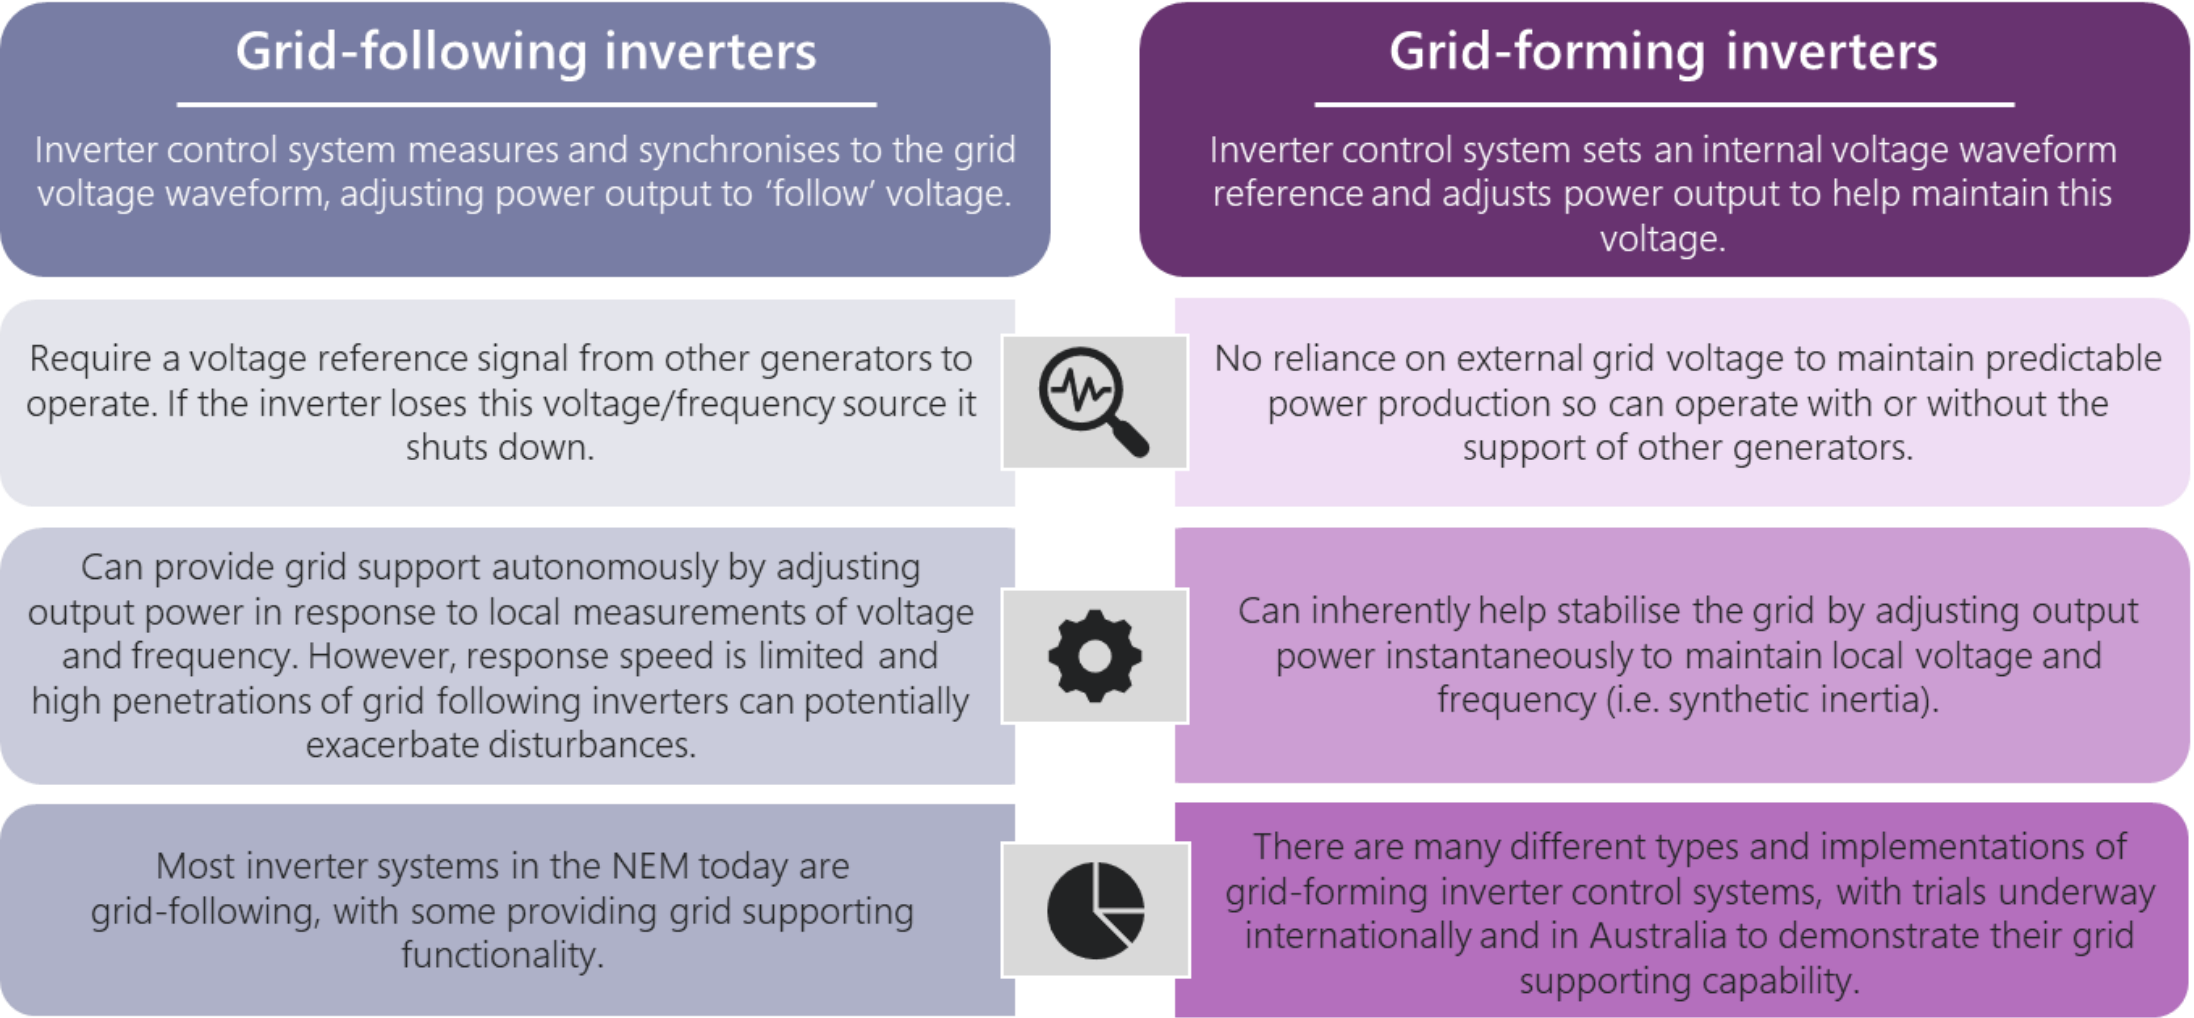
\includegraphics[width=14cm]{images/gfli_vs_gfmi.png}
    \caption{Differences between grid-following and grid-forming
    \cite{taylor2021application}.}
    \label{fig:gfli_vs_gfmi}
\end{figure}

% TODO: mention the importance of the non-saliency of SMs, and also the
% importance of the dynamics of the damper windings.
One of the most popular GFMI control approaches is based on introducing the SG
dynamic models into the controllers of the inverter, enabling it to operate like
a rotating electrical machine. This control approach is known as Virtual
Synchronous Machine (VSM), and implementations of different orders have been
reported in the literature, ranging from detailed electromechanical models
\cite{beck2007vsm}\cite{zhang2013vsm} to simplified swing dynamics
\cite{zhong2011synchronverter}\cite{alipoor2015power}. However, there is still
little literature discussing the necessity of detailed electromechanical models,
and models of intermediate complexity, such as the 1-axis (flux-decay) model,
have not been reported yet \cite{chen2020modeling}.

\section{Objectives}
This thesis focuses on the modeling, simulation, and analysis of VSMs of
different orders in a multi-machine power system with multiple SGs. The main
goals of this project are to evaluate the necessity of detailed
electromechanical models when implementing VSMs and to propose a VSM model
equivalent to the 1-axis (flux-decay) SG model. The entire work is divided into
the following steps:

\begin{enumerate}
    \item Study of the modeling and simulation of voltage source power converters;
    \item Study of the multiple implementations of VSMs; 
    \item Comparison between VSMs of multiple orders and 2-axis (subtransient)
    model of SG in terms of frequency deviation and output voltage and power
    under load increase and ground fault.
\end{enumerate}
% TODO: improve the objectives, write something like the following
% • To build up a control strategy of conventional generator without alteration, where
% voltage and frequency are controlled by the AVR and governor respectively.
% • Study and develop electronic control methodologies to provide additional inertia
% to microgrid for the better dynamic stability of the system.
% • Design and implement suggested control methodologies for island microgrid
% connected with both real power and reactive power load
% • Investigate the designed control system with different types of load to determine
% how it plays a role in system stability in the presence of various disturbances.
% • Review the existing methodology on VSM, analyze system design and operation,
% and explore the scope and limitation.

% TODO: structure of the thesis might need to be revised
\section{Strcture of the Thesis}
The remainder of this thesis is organized as follows. In Chapter 2, we present
an overview of the main implementations of VSMs in the literature, from detailed
electromechanical models to simplified swing dynamics. In Chapter 3, we present
a detailed mathematical modeling of voltage source converters, and their
controllers enabling the VSMs dynamics. Chapter 4 presents the. In the Appendix,
we describe the modeling and simulation methods of main power system components
such as SMs, loads and transmission lines.